
\footnotetext{Este capítulo se toma en gran parte de la tesis doctoral del autor. University of Alberta, 2007.El texto completo está disponible en \url{personal.inb.unam.mx/lconcha}. El autor agradece a Penélope Martínez Campos por la traducción del texto original.}

\section{Difusión de moléculas de agua}

Todas las moléculas con una temperatura por encima del cero absoluto (es decir, $>$-273.15 \degrees) están en movimiento constante. Este fenómeno fue descrito por primera vez en 1828 por Robert Brown \cite{Brown1828}, basado en la observación del movimiento aleatorio de los granos de polen suspendidos en el agua. Aunque los granos de polen son considerablemente más grandes que las moléculas individuales, el comportamiento descrito por Brown es similar al observado en las moléculas \footnote{De hecho, el movimiento de los granos de polen fue secundario a la difusión del agua moléculas en las que fueron suspendidas.}, por lo tanto, el fenómeno molecular se denomina comúnmente movimiento browniano. La difusión es accionada térmicamente y en el caso más simple es completamente estocástica, con cada molécula describiendo una ``caminata aleatoria'' en el tiempo. Por ejemplo, si una sola molécula de agua suspendida en un mar infinito de agua tranquila pudiera ser seguida a través del tiempo, el camino parecería ser completamente al azar, con probabilidades iguales de ir a cualquier lugar en cada paso del tiempo. Cuanto más tiempo observamos, más lejos podría estar la molécula de agua desde donde comenzó. Sin embargo, con probabilidades iguales de moverse en cualquier dirección, el desplazamiento promedio en el tiempo sería cero.

Albert Einstein resolvió matemáticamente las observaciones de Brown \cite{Einstein1905}. Consideremos varias moléculas de agua que se difunden libremente, cada una con una posición inicial $r$ en el tiempo {$t = 0$}. Si permitimos que  difundan durante un período de tiempo \(\tau\), cada molécula de agua estará entonces en la posición {$r'$}. El coeficiente de difusión {$D$} se puede encontrar por:
Albert Einstein resolvió matemáticamente las observaciones de Brown \cite{Einstein1905}. Consideremos varias moléculas de agua que se difunden libremente, cada una con una posición inicial $r$ en el tiempo {$t = 0$}. Si permitimos que  difundan durante un período de tiempo \(\tau\), cada molécula de agua estará entonces en la posición {$r'$}. El coeficiente de difusión {$D$} se puede encontrar por:

\begin{equation}
D = \frac{1}{6 \tau}  \langle \textbf{R}^T\textbf{R} \rangle
\end{equation}

donde $\textbf{R}$ = {$r'- r$}. El desplazamiento del spin (de los protones en el agua) en el tiempo se considera sobre el conjunto de spins (paréntesis angulados). El desplazamiento en el tiempo {$t$} está dado por la raíz cuadarada del promedio de los desplazamientos al cuadrado ($rms$, por sus siglas en inglés):

\begin{equation}
rms_{n} = \sqrt{2nDt}
\end{equation}
donde {$n$} es el número de dimensiones. El desplazamiento de moléculas de agua en una dimensión se ejemplifica en la Figura \ref{fig:difusion_gaussian} \\

\begin{figure}[htb]
	\begin{figg}
    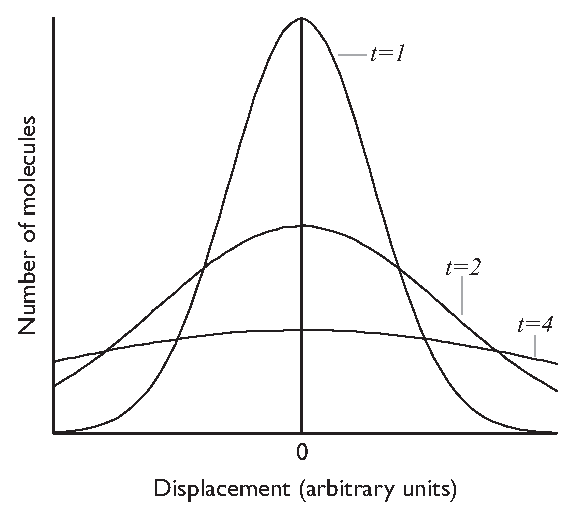
\includegraphics[width=0.7\textwidth]{gaussianDiffusion.eps}
    \caption{\textbf{Desplazamiento unidimensional de moléculas de agua en el tiempo.} Un número arbitrario de moléculas de agua con posición = 0 en $t = 0$ se difunde con el tiempo. El perfil de desplazamiento gaussiano se amplía a medida que pasa el tiempo.}
    \label{fig:difusion_gaussian}
    \end{figg}
\end{figure}

Recuerde que la difusión es aleatoria (es decir, isotrópica) y, por lo tanto, $D$ es no depende de la dirección a la que se dirige. La magnitud de $D$ depende de la viscosidad y temperatura del medio, y del tamaño de la molécula. El $D$ de agua a 37 \degrees es alrededor de 3.04×10\textsuperscript{-3} mm\textsuperscript{2}/s.\cite{Mills1973}

En el caso de las moléculas de agua, el soluto y el disolvente son la misma molécula, y el fenómeno se denomina autodifusión, para lo cual el modelo de caminata aleatoria simple puede predecir adecuadamente su comportamiento. Ejemplos de auto-difusión de las moléculas de agua se pueden ver en la Figura 2.2. Para el resto de este documento, el término \emph{difusión} se emplea para referirse a la auto-difusión de moléculas de agua.

\begin{figure}
	\begin{figg}
    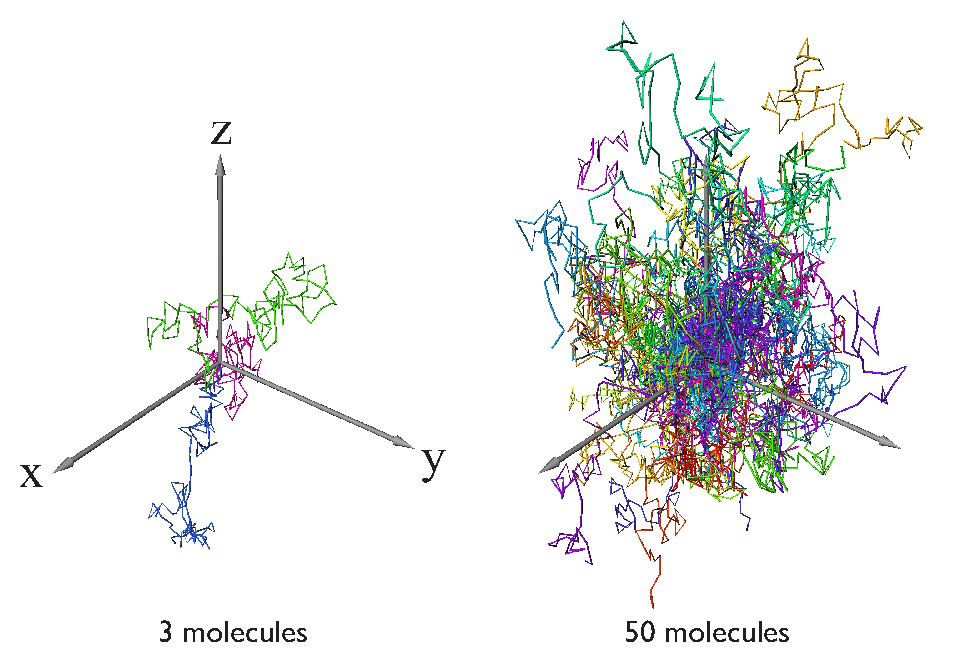
\includegraphics [width=0.7\textwidth]{isotropicExamples.eps}
    \caption{\textbf{Simulación de caminata aleatoria sobre 100 pasos de tiempo de 3 y 50 moléculas de agua.} La dirección de cada molécula se define aleatoriamente en cada paso. Con el tiempo, las moléculas de agua tienen una probabilidad no nula de visitar cualquier posición en el espacio, pero, en promedio, han movido poco con respecto al origen.}
    \end{figg}
\end{figure}

\subsection{Medición de la difusión con resonancia}

Los efectos de la difusión sobre la señal de RMN se conocen desde la década de 1950, cuando el spin-eco fue descrito por Hahn \cite{Hahn_1950}. Algunos años más tarde, Carr y Purcell publicaron su trabajo sobre medidas cuantitativas T2, en las que reconocen la importancia de la difusión e incluso miden $D$ en una muestra de agua \cite{Carr_1954}. En 1956, Torrey modificó las ecuaciones de Bloch para incluir un término de difusión \cite{Torrey_1956}. Estos primeros intentos de medir $D$ se basaron en el uso de una perturbación constante del campo magnético principal que, entre otros problemas, dificultó la distinción de los efectos relacionados a $D$ de aquellos provocados por la relajación transversal \Ttwo.

Fue el trabajo de Stejskal y Tanner \cite{Stejskal_1965} en los años sesenta lo que facilitó la medición cuantitativa de los coeficientes de difusión molecular mediante el uso de una secuencia de eco de spin con gradientes pulsados (PGSE, Figura \ref{F:stejskal_sequence}). La idea básica es codificar la posición espacial de las moléculas de agua (spins) en $t = 0$, invertir la fase de spin con un pulso $\pi$ y decodificar la posición del spin después del tiempo $\tau$. La posición de los spins (moléculas de agua) es codificada y recodificada con el uso de gradientes de campo magnético (Figura 2.3). Con más detalle: Después de la aplicación de un impulso de radiofrecuencia $\pi/2$ que coloca la magnetización neta en el plano \Mxy con fase cero, se activa un gradiente de campo magnético con amplitud $G$ y duración $\delta$, lo que imparte una fase a los spins según su posición espacial. Como en cualquier eco de spin, un pulso de radiofrecuencia con ángulo $\pi$ (180 \degrees) provoca el refasamiento del ensamble de spins. Un segundo gradiente de campo magnético con las mismas características que el primero (con una separación $\Delta$ con respecto al primero) hace que los spins estáticos (los que no se movieron en el espacio entre ambos pulsos de gradiente) recuperen su fase original. El eco se adquiere en este punto. Si los spins se mueven durante el tiempo entre los dos gradientes del campo magnético (debido a la difusión o a cualquier otra causa), los giros no podrán refasarse completamente, lo que hace que se obtenga menos señal de RMN. Obsérvese que los gradientes de campo se aplican linealmente en una dimensión, proporcionando sensibilización a la difusión sólo a spins que se mueven en esa dirección particular. Es decir, si un spin se mueve perpendicularmente a la dirección del gradiente del campo, no contribuirá a la pérdida de la señal de RMN. La señal puede ser adquirida a través de un eco de spin, como se ha descrito anteriormente, o a través de un eco estimulado \cite{Tanner_1970}. Este último enfoque, que está fuertemente ponderado a \Tone, minimiza la pérdida de señal a través de la relajación transversal, aunque su propia naturaleza se traduce en una reducción del 50\% de la señal original disponible. Se puede también obviar el pulso de radiofrecuencia con ángulo $\pi$, convirtiendo a la secuencia en un eco de gradiente; en este caso el segundo pulso de gradiente debe tener la orientación opuesta al primero ($+G/-G$). Como se revisó en el Capítulo \ref{chapter_relajacion}, los ecos de gradiente proveen menor cantidad de señal, por lo que es mucho más habitual el uso de ecos de spin cuando se codifica la difusión.

Mediante la modificación de las características de la secuencia PGSE, se puede aumentar o disminuir la sensibilidad a la difusión. Si la amplitud de los gradientes se incrementa ($G$), los spins requerirán menos movimiento para experimentar un campo magnético diferente, aumentando así el cambio de fase. Alternativamente, se puede permitir que los spins difundan durante un período de tiempo más largo, aumentando la probabilidad de que los spins se desfasen entre ellos. El tiempo de difusión se expresa como $\Delta - \delta/3$, donde la corrección $\delta/3$ explica la difusión que se produce durante el tiempo en que los gradientes se ejecutan \cite{Stejskal_1965}. La sensibilidad a la difusión se expresa como:
\begin{equation}
b = \gamma^2G^2\delta^2 (\Delta - \frac{\delta}{3})
\label{eq:bval}
\end{equation}
donde $\gamma$ es la relación giromagnética de protones de hidrógeno (42,58 MHz/T). La ecuación \ref{eq:bval} supone que los gradientes de campo local (independiente de los gradientes de difusión-sensibilización) son mínimos en la muestra. En áreas de grandes diferencias de susceptibilidad magnética, se inducen gradientes de campo magnético local. Los gradientes locales impartirían más desplazamientos de fase al spin que no serían totalmente recuperados por el segundo pulso de gradiente, confundiendo la medición de $D$. Cualquier otro gradiente de campo magnético o inhomogeneidad presente durante la secuencia de PGSE debe estar presente y ser idéntico durante la aplicación de ambos gradientes de sensibilización de difusión para poder inferir $D$ correctamente. El límite de tejido entre el aire y el tejido es un ejemplo de este problema (más sobre esto en la Sección \ref{sec:ArtefactosDWI}). Los gradientes sensibilizadores de difusión no tienen que ser rectangulares, como se expresa en la ecuación anterior, en cuyo caso el área del pulso debe ser igual a la del impulso rectangular ideal. El uso de pulsos de gradiente no rectangulares no afecta a la medición de $D$.\cite{Price_1991}

\begin{figure}
	\begin{figg}
    \includegraphics [width=0.7\textwidth] {stejskal_sequence.eps}
    \caption{\textbf{Secuencia de eco de spin con gradientes pulsados (PGSE).} La posición espacial de las moléculas de agua se codifica como fase mediante el uso de un gradiente de campo magnético con duración $\delta$ y magnitud $G$. Un pulso $\pi$ invierte la fase de spin. Un segundo gradiente de campo magnético, idéntico al primero, reenfoca la fase de todos los giros estacionarios. Los giros móviles no experimentan el mismo campo magnético antes y después del pulso $\pi$ de reorientación y el conjunto no se reenfoca homogéneamente, dando como resultado la pérdida de la señal.}
    \label{F:stejskal_sequence}
    \end{figg}
\end{figure}

La cantidad de señal de RMN disponible en un experimento sensible a la difusión decae exponencialmente de acuerdo con $D$ (Figura \ref{F:expDecay_signal_b_2panels}), y se expresa como:

\begin{equation}
\label{eq:bexpdecay}
\frac{S}{S_0} = e^{-bD}
\end{equation}

donde $S$ es la intensidad de señal obtenida con el gradiente de difusión activado y $S_0$ es la intensidad de señal correspondiente obtenida sin el uso de gradientes sensibilizadores de difusión. Esta ecuación también puede expresarse linealmente como:

\begin{equation}
\label{eq:blindecay}
ln (\frac{S}{S_0}) = -bD
\end{equation}\\

\begin{figure}
	\begin{figg}
    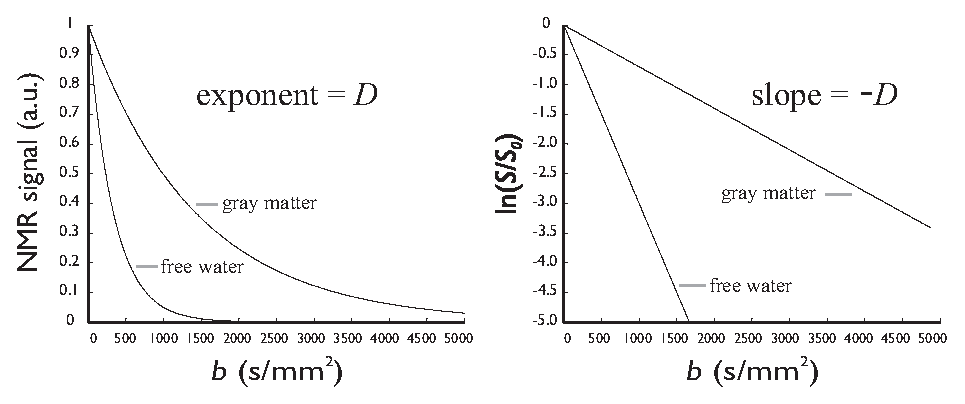
\includegraphics [width=0.7\textwidth] {expDecay_signal_b_2panels.eps}
    \caption{\textbf{Señal de RMN de acuerdo al nivel de sensibilización a difusión.} La señal de RMN se representa como una función de $b$ (ecuación \ref{eq:bval}). Se muestran señales de sustancia gris ($D$ = 0.7×10\textsuperscript{-3} mm\textsuperscript{2}/s y agua que difunde libremente a 37\degrees C ($D$ = 3×10\textsuperscript{-3} mm\textsuperscript{2}/s). El panel izquierdo muestra el decaimiento exponencial de la señal en función de $b$ (ecuación \ref{eq:bexpdecay}), mientras que la versión lineal (ecuación \ref{eq:blindecay}) se muestra en el panel derecho.}
    \label{F:expDecay_signal_b_2panels}
    \end{figg}
\end{figure}

Aunque originalmente se desarrolló para medir $D$ en muestras, el PGSE y sus variantes pueden usarse en IRM. En este caso, el volumen de interés se divide en $n$ píxeles (elementos de imagen en el caso bidimensional) o voxeles (elementos de volumen, en el caso tridimensional), y el coeficiente de difusión se puede calcular en cada pixel individual o voxel. Dado el impacto que tiene la difusión en el contraste de la imagen resultante, a estas imágenes se les conoce como imágenes ponderadas (o sensibles) a difusión (\textit{diffusion-weigted images}, DWI, en inglés) \cite{Wesbey_1984} y ahora se utiliza de forma rutinaria en la detección de lesión cerebral isquémica \cite{Sotak_2002}. Los gradientes de sensibilización a la difusión, así como los pulsos de radiofrecuencia, deben estar encendidos durante un cierto tiempo, proporcionando un tiempo de difusión efectivo $\Delta - \delta/3$) que es de alrededor de 50-100 ms. En los tejidos biológicos, la difusión de las moléculas de agua depende no sólo de la viscosidad y la temperatura, sino también de las barreras semipermeables como las membranas celulares. Para medir la viscosidad, el tiempo de difusión debe ser muy corto, limitando las interacciones entre las moléculas de agua y las barreras semipermeables. Tales cortos tiempos de difusión son difíciles de alcanzar ya que requieren gradientes $G$ muy poderosos que se aplicarán durante un brevísimo período de tiempo $\delta$). Tanner y Stejskal \cite{Tanner_1968} reconocieron el efecto de las barreras de difusión y fueron los primeros en proponer la idea de medir la difusión restringida de moléculas de agua al variar el tiempo entre los pulsos de gradiente ($\Delta$). Por lo tanto, las DWI no acceden a $D$, sino que brindan información acerca de cómo el tejido modula la señal. Por esta razón, el término Coeficiente de Difusión Aparente (CDA, o ADC por sus siglas en inglés) se utiliza cuando se hace referencia a $D$ en los tejidos biológicos medido con RMN. Afortunadamente, esto está lejos de ser un inconveniente, ya que la parte {\emph aparente} de ADC es lo que nos permite hacer inferencias sobre la microestructura de los tejidos.


En DWI se utiliza un par de gradientes sensibilizadores de difusión antes del esquema de adquisición de imágenes. Es decir, los gradientes sensibilizadores a difusión (con duración $\delta$) son totalmente independientes de los gradientes que se utilizan para la codificación espacial (Capítulo \ref{chapter_espacial}). Aunque puede utilizarse cualquier esquema de condificación espacial, la más frecuentemente utilizada es el método de imagen ecoplanar (EPI) \cite{Mansfield_1977,Ordidge_1988}, ya que es uno de los esquemas de imagen más rápidos disponibles en la RM. En EPI, se utiliza un único impulso de excitación y cada DWI se forma en menos de un cuarto de segundo por rebanada (ver ejemplos en Figura \ref{F:DTI_DWItoTensor}). Los gradientes de difusión se aplican en una dimensión, por lo tanto sensibilizando la imagen a la difusión en una dirección (además de la contribución de \Ttwo que resulta inevitable por los TE largos que se requieren para que logren desarrollarse los gradientes de difusión con duración $\delta$).\footnote{Si esto resulta confuso, se invita a la lectura del Capítulo \ref{chapter_relajacion}.} Las regiones de las imágenes que contienen la mayor parte de sus moléculas de agua difundiendo en una dirección que es paralela a la dirección del gradiente de difusión mostrarán una disminución de la señal, cuando se compara con la imagen no sensible a difusión. Por lo tanto, el ADC de esas regiones será alto. Por el contrario, las regiones donde la difusión es perpendicular a los gradientes de difusión no mostrará una caída tan marcada en la intensidad de la señal. Nótese que entonces una misma región anatómica puede mostrarse hiperintensa en una DWI, e hipointensa en otra DWI con sensibilización a otra dirección. Habiendo calculado el ADC por pixel, se pueden producir mapas cuantitativos de difusividad donde la escala de grises está relacionada con ADC, como en la Figura \ref{F:DTI_ADCmaps}. Es importante señalar que las áreas de hiper-intensidad visto en DWI suelen aparecer como regiones oscuras en los mapas cuantitativos ADC. Las primeras imágenes de DWI fueron presentadas en 1988 por Avram y Crooks \cite{Avram_1988}. Sin duda, las DWI han tenido un tremendo impacto en el diagnóstico de lesiones cerebrales isquémicas, donde se ha convertido en una herramienta virtualmente indispensable \cite{Sotak_2002,Moseley_1990a,Warach_1995}.

\begin{figure}
\begin{figg}
   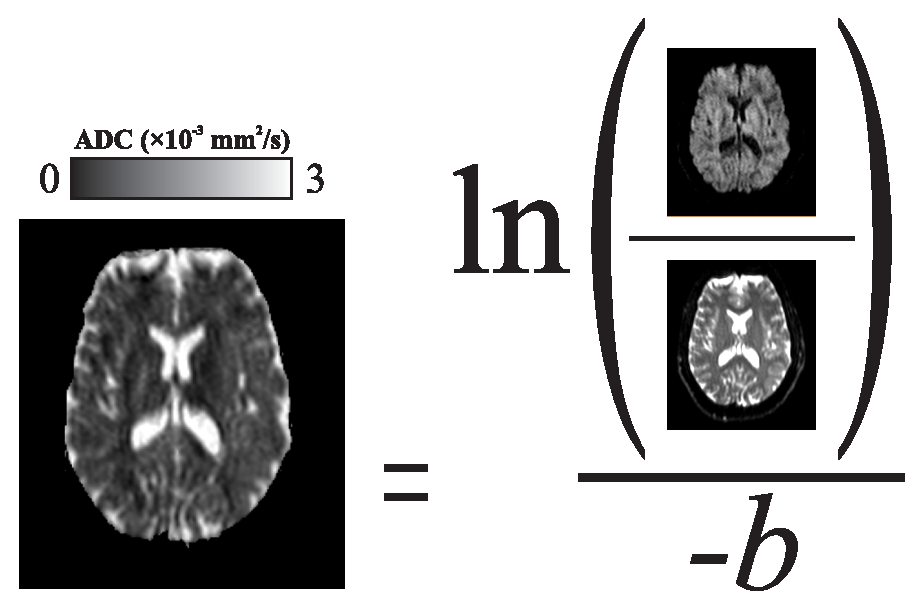
\includegraphics [width=0.7\textwidth] {DTI_ADCmaps.eps}
    \caption{\textbf{Mapa del coeficiente de difusión aparente cuantitativo.}
    El ADC se calcula sobre una base de píxel a píxel de la DWI y las imágenes
    ponderadas de no difusión de acuerdo con la ecuación \ref{eq:blindecay}. El gradiente de difusión se aplica en una sola dirección; $b = 1000 s/mm^{2}$. Observe la rápida difusión de FCE en los ventrículos, representada como píxeles  brillantes en el mapa de ADC cuantitativo.}
        \label{F:DTI_ADCmaps}
    \end{figg}
\end{figure}


\subsection{Difusión de agua en el cerebro}

Con el fin de comprender el comportamiento de la
difusión de agua en el cerebro, debemos discutir brevemente las propiedades
básicas de los cuatro tipos principales de tejidos que residen en la
cavidad intracraneal:

\begin{description}
\item[Substancia gris (SG)] Este tejido contiene los cuerpos neuronales y las células gliales. Tiene un color gris-marrón, de ahí su nombre, y se distribuye en la superficie de los hemisferios cerebrales y cerebelo, así como los núcleos subcorticales (tálamo, caudado, etc.). Se compone de más de 100 000 millones de neuronas, y un número aún mayor de células gliales. Alrededor del 90\% de todas las neuronas del cerebro residen en la corteza cerebral \cite{Pakkenberg_1997}, que tiene un grosor de alrededor de 1-5 mm y se organiza en capas. Representa el 45\% del volumen total del cerebro en la edad adulta joven \cite{Rengachary_2004}.
\item[Substancia blanca (SB)] Compuesta de axones y oligodendrocitos, proporciona conexiones entre porciones cercanas y distantes del cerebro. Su color es debido al alto contenido de mielina. En adultos jóvenes, tiene un volumen aproximado de 450 cm\textsuperscript{3} (35\% del volumen cerebral) y los axones mielinizados por sí solos representan más de 118 000 km \cite{Tang_1997}.
\item[Líquido céfalorraquídeo (LCR)] Con un volumen total inferior a 150 ml, este líquido transparente baña el cerebro y la médula espinal, siendo intercambiado completamente 3-4 veces al día. Es 99\% de agua, y tiene menos de 10 células por mm\textsuperscript{3} \cite{Kandel_2000}. Representa el 10\% del volumen cerebral total \cite{Rengachary_2004}.
\item[Sangre] El flujo sanguíneo a través del cerebro entero en un adulto joven es del 15-20\% del gasto cardíaco, entre 750-1000 ml/min \cite{Kandel_2000}. Representa alrededor del 10\% del volumen total del cerebro \cite{Rengachary_2004}.
\end{description}

La difusión de agua no es completamente libre en los sistemas biológicos, debido a la presencia de membranas celulares y organelos, así como a la arquitectura tisular característica. Estas características presentan barreras a la difusión y causan {\emph anisotropía} (es decir, la difusión no es igual en todas las direcciones). La substancia blanca en el cerebro, que consiste en varios haces de axones que interconectan distantes porciones discretas del cerebro, muestra un alto grado de coherencia en su arquitectura tisular. Por lo tanto, muestra el mayor nivel de anisotropía en el cerebro.

Los axones con trayectorias similares se agrupan para formar fascículos (también denominados tractos o haces de fibras, Figura \ref{F:axons2}). Cada axón puede estar rodeado varias veces por vainas de mielina ricas en lípidos, producidas por oligodendrocitos. Las vainas de mielina se interrumpen periódicamente a lo largo del axón en los nodos de Ranvier, obligando a la propagación de los potenciales de acción a ser saltatoria y por lo tanto más rápida. Los diámetros de los axones varían desde $1 \mu$m hasta aproximadamente 15 \(\mu\)m. Dado el coeficiente de difusión de las moléculas de agua a la temperatura corporal, una sola molécula de agua puede mostrar un desplazamiento de alrededor de 10 \(\mu\)m en 50-100 ms (tiempo de difusión habitual en las DWI) \cite{Le_Bihan_2002}, sin duda, suficiente para que encuentre varias membranas axonales y otras barreras. La mielina, que es una bicapa lipídica, fue asumida erróneamente como la única fuente de anisotropía de difusión. La anisotropía está efectivamente presente en los nervios no mielinizados \cite{Beaulieu_1994,Gulani_2001}, pero la presencia de mielina modula el grado de anisotropía \cite{Gulani_2001,Tyszka_2006}. La anisotropía en los nervios no mielinizados apunta a membranas celulares intactas como una de las principales fuentes de anisotropía de las moléculas de agua \cite{Beaulieu_1994,Gulani_2001}. Los micro-túbulos orientados longitudinalmente dentro de los axones, así como el transporte axonal rápido, parecen estar mínimamente involucrados en la generación de anisotropía de difusión \cite{Beaulieu_1994}. Cuando los axones están organizados de forma coherente y bien ceñidos, como en los fascículos o haces, se combinan los efectos impermeables de las vainas de mielina y las membranas axonales, lo que hace que las mediciones generales de difusión de la sustancia blanca sean anisotrópicas. Los mecanismos biofísicos de la anisotropía de difusión han sido previamente revisados \cite{Beaulieu2002}.

La substancia gris, aunque está organizada en capas y columnas funcionales, no muestra el mismo grado de coherencia arquitectónica que la SB. El neuropilo (las dendritas y axones que interconectan los cuerpos neuronales \emph {dentro} de la corteza), en particular, está enredado y no muestra una arquitectura coherente. Por esta razón, la difusión de agua en la corteza no muestra un alto grado de anisotropía. El LCR, siendo esencialmente agua, muestra una difusión rápida e isotrópica. Por último, la difusión del agua en la sangre es difícil, si no imposible, de medir dado el flujo rápido que ocurre simultáneamente.

\begin{figure}
	\begin{figg}
    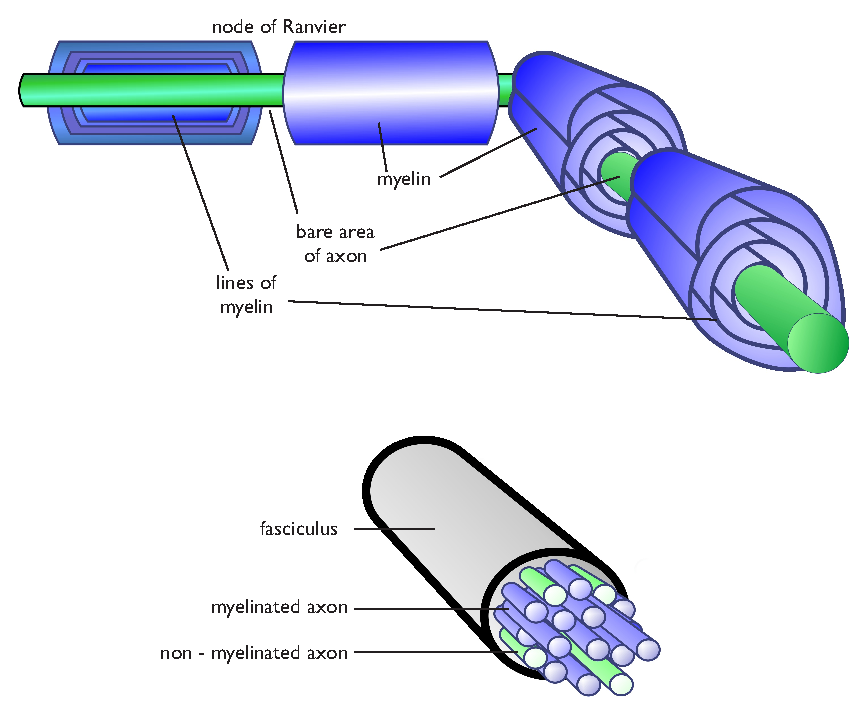
\includegraphics [width=0.7\textwidth] {axons2.eps}
    \caption{\textbf{Estructura básica de la substancia blanca.} Algunos axones son envueltos en forma de espiral por extrusiones del citoplasma de oligodendrocitos, formando las vainas de mielina. El aislamiento de mielina se interrumpe en los nodos de Ranvier. Los axones mielinizados y no mielinizados se agrupan en fascículos con estructura interna altamente homogénea.}
    \label{F:axons2}
    \end{figg}
\end{figure}

\section{El tensor de difusión}

Dada la anisotropía de la difusión en los tejidos organizados, una medida escalar como $D$ no es suficiente para representar el perfil tridimensional del movimiento de las moléculas de agua. En el caso más simple, en el que se conoce {\emph a priori} la orientación del tejido, tal como un nervio periférico, es posible cuantificar la anisotropía de difusión midiendo el ADC usando gradientes de sensibilización a la difusión orientados tanto en paralelo como en perpendicular al tejido y obteniendo el relación entre los dos ($\mbox{anisotrop\'ia} = (\frac{ADC\parallel}{ADC\perp})$). Sin embargo, la orientación del tejido, por lo general, no se conoce de antemano, como es el caso de la sustancia blanca. Basser y sus colegas introdujeron el formalismo del tensor de difusión en 1994 \cite{Basser_1994_2,Basser_1994}, que supera dicho problema y permite la cuantificación del CDA en cualquier dirección. Lo más importante es que el tensor de difusión proporciona información importante sobre la microestructura y la orientación del tejido organizado. La representación tridimensional de la ecuación \ref{eq:blindecay} es:
\begin{equation}
\begin{array}{l}
ln(\frac{S}{S_0}) = \sum_{i=1}^{3}\sum_{j=1}^{3} b_{ij}D_{ij} \\
                  = (-b_{xx}D_{xx}+2b_{xy}D_{xy}+2b_{xz}D_{xz}+b_{yy}D_{yy}+2b_{yz}D_{yz}+b_{zz}D_{zz})
\end{array}
\end{equation}
que podemos expresar de manera más compacta como matriz:
\begin{equation}
ln \bigg(\frac{S(\textbf{b})}{S_0}\bigg) = -traza(\textbf{bD})
\end{equation}
donde cada elemento en $\textbf{b}$ y $\textbf{D}$ corresponde a una dirección unidimensional particular de sensibilización por difusión. A partir de estas ecuaciones, el tensor puede construirse como matriz de la forma:

\begin{equation}
\textbf{D}
=
\begin{bmatrix}
    D_{xx} & D_{xy} & D_{xz} \\
    D_{xy} & D_{yy} & D_{zy} \\
    D_{xz} & D_{yz} & D_{zz}
\end{bmatrix}
\end{equation}
Obsérvese que $\textbf{D}$ es una matriz simétrica, donde $D_{xy}, D_{xz}$ y $D_{yz}$ son repetidos en las esquinas superior derecha e inferior izquierda, ya que $D_{xy} = D_{yx}$, $D_{xz} = D_{zx}$, y $D_{yz} = D_{zy}$. Si el medio es isotrópico, entonces $D{xx} = D{yy} = D_{zz}$, y los elementos fuera de la diagonal, $D_{xy}, D_{xz}$ y $D_{yz}$ son cero.  Si el la difusión es anisotrópica, los elementos fuera de la diagonal pueden adquirir valores positivos o negativos, y representan la covarianza que existe entre los ejes $x$, $y$, y $z$. Dado el número de incógnitas en la construcción de \textbf{$D$}, se requiere la obtención de, al menos, 6 mediciones $S$ en direcciones distintas, y una señal $S_0$. En términos de imagen, se requiere una imagen no sensible a difusión ($b=0$ s/mm$^2$) y por lo menos 6 DWI ($b>0$ s/mm$^2$) que estén sensibilizadas a la difusión en 6 direcciones distintas. Es común adquirir muchas más que 6 DWI, y utilizar un método de mínimos cuadrados para inferir el tensor. Esta estrategia permite la estimación más precisa del tensor, pues al incrementar el número de mediciones se promedia el ruido entre ellas \cite{Jones_2004}. Existen además muchos algoritmos que realizan el ajuste del tensor de forma no lineal, o de manera robusta a datos extremos \cite{chang2005restore,mangin2002distortion}.



% \begin{figure}
%   \begin{minipage}[c]{0.45\linewidth}
%     
%     \begin{adjustbox}{width=\columnwidth-100pt}
%     \begin{tabular}{ lll }%
%       \multicolumn{3}{c}{{\it x} \hfill	$y$ \hfill $z$} \\%
%       \hline 
%       1 & 0 &  1 \\ 
%      -1 & 0 &  1 \\ 
%       0 & 1 &  1 \\ 
%       0 & 1 & -1 \\ 
%       1 & 1 &  0 \\
%      -1 & 1 &  0
%     \end{tabular}%
%     \end{adjustbox}
%     \vspace{0pt}
%   \end{minipage} 
%   \begin{minipage}[c]{0.55\linewidth}
%     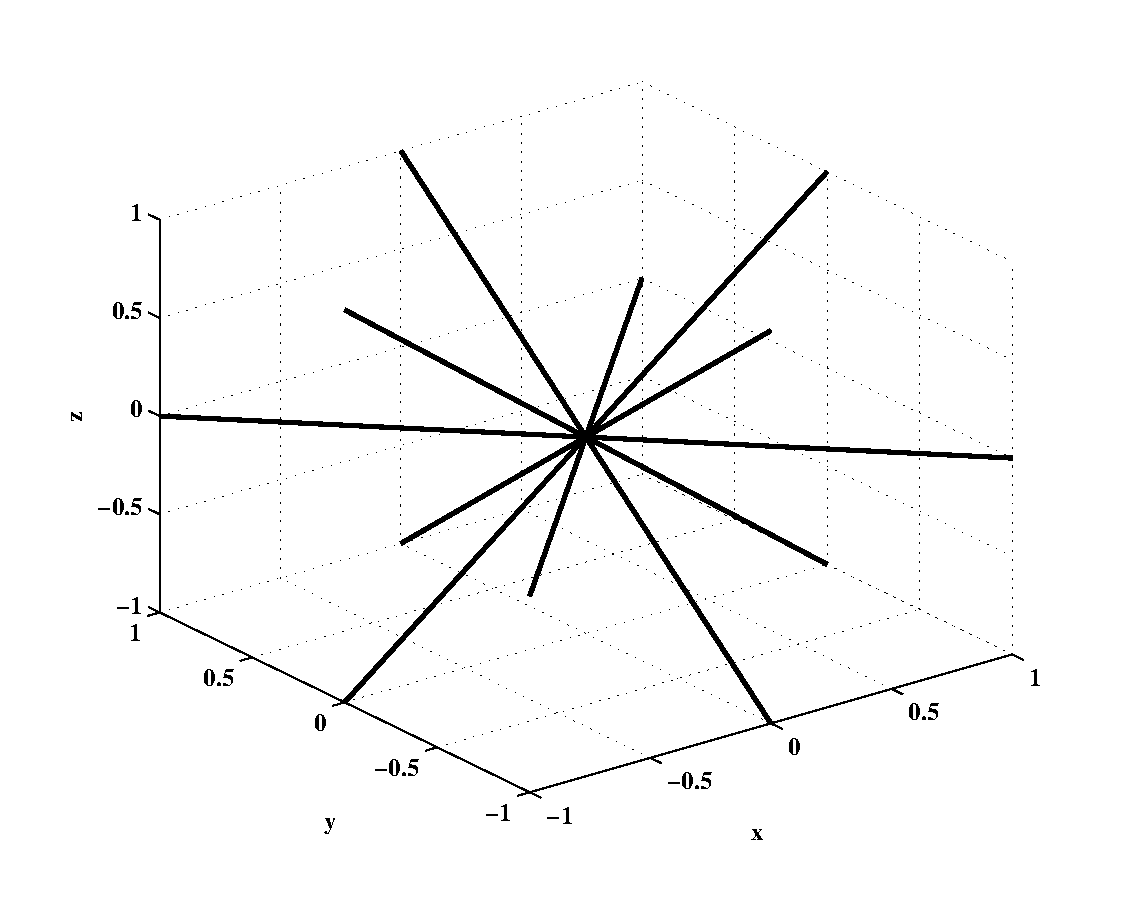
\includegraphics[width=1\textwidth, inner] {bmatrix.eps}
%     \vspace{0pt}
%   \end{minipage}% 
%   \caption{\textbf{Direcciones de gradiente de difusión.} Las direcciones de gradiente de difusión se trazan en tres dimensiones. Las imágenes ponderadas por difusión se obtienen en seis direcciones de gradiente de difusión no planar y no colineal con el fin de obtener suficiente información para construir el tensor de difusión.}
% \label{bmatrix}
% \end{figure}

Una propiedad de los tensores de segundo rango es que pueden ser diagonalizados, dejando tres elementos distintos de cero a lo largo de la diagonal principal de la matriz, que se llaman valores propios.\footnote{Las y los lectores familiarizados con métodos de reducción de dimensionalidad habrán notado que el ajuste del tensor es un caso particular del análisis de componentes principales.} Los valores propios se ordenan según su magnitud, siendo \lone el más grande y \lthree el más pequeño en magnitud. La relación matemática entre las coordenadas principales del tensor de difusión y el marco del laboratorio se describe por los vectores propios ($\nu_{1-3}$). Los valores propios (autovalores o {\emph eigenvalues}) reflejan la difusividad en una dirección dada, de acuerdo con su vector propio asociado y tienen interpretaciones biológicas directas. Por ejemplo, en el caso de la sustancia blanca, el autovalor más largo (es decir, \lone) refleja el estado axonal, mientras que los valores propios asociados a ($\nu_{2,3}$) proporcionan información sobre la integridad de las vainas de mielina \cite{Song_2003,Concha_2006}).

Es más fácil entender el tensor de difusión al considerar su representación geométrica, que es un elipsoide cuyos ejes están determinados por los tres valores propios y su orientación por los vectores propios (Figura \ref{F:DTI_ellipsoid}). El elipsoide puede ser conceptualizado como la superficie sobre la cual un spin en el origen se difundirá con igual probabilidad si la difusión es gaussiana. La superficie del elipsoide representa el desplazamiento (rms) del agua. La traza del tensor (traza ($\textbf {D}) = \lambda_1 + \lambda_2 + \lambda_3)$ es equivalente al tamaño del elipsoide, mientras que la difusividad media en todas las direcciones (ADC tridimensional) está dada por:
\begin{equation}
ADC = \frac{traza (\textbf{D})}{3} = \frac{\lambda_{1} + \lambda_{2} + \lambda_{3}}{3}
\end{equation}
Los términos difusividad media (DM), $traza/3$ y ADC se utilizan indistintamente en la literatura. $Traza$ ADC también se utiliza a veces para referirse a DM, aunque se refiere formalmente a ADC$\times 3$.

\begin{figure}
	\begin{figg}
    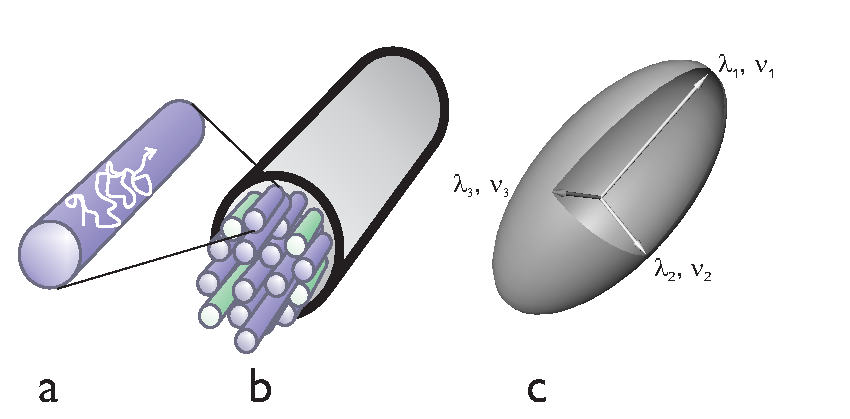
\includegraphics [width=0.7\textwidth] {DTI_ellipsoid.eps}
    \caption{\textbf{El tensor de difusión.} La difusión anisotrópica de moléculas de agua (a) en tejidos altamente organizados, como la materia blanca (b), da como resultado un tensor de difusión alargado, visualizado como un elipsoide (c). El eje mayor del elipsoide corresponde al valor propio más grande ($\lambda_1$). Por lo tanto, la difusividad principal de las moléculas de agua es paralela al vector propio correspondiente a $\lambda_1$.}
    \label{F:DTI_ellipsoid}
    \end{figg}
\end{figure}

Las imágenes del tensor de difusión (DTI, por sus siglas en inglés) representan la reconstrucción, a partir de al menos 6 DWI y una imagen no sensible a difusión, de un tensor de difusión por cada voxel en el volumen. 


Las DWI son inherentemente sensibles a la difusión de forma unidimensional. Obteniendo al menos seis DWI, cada uno con una dirección de gradiente de difusión diferente (no colineal y no coplanar) (y una imagen sin sensibilización por difusión, $b = 0 s/mm^{2}$), y obteniendo sus respectivos mapas ADC en una dirección de gradiente de pixel por pixel, adquirimos toda la información necesaria para construir el tensor de difusión, dando lugar a imágenes de tensor de difusión (Figura \ref{F:DTI_DWItoTensor}).

\begin{figure}
	\begin{figg}
    \includegraphics [width=0.7\textwidth]{DTI_DWItoTensor.eps}
    \caption{\textbf{Cálculo del tensor de difusión.} El tensor de difusión se calcula píxel a píxel, basado en la imagen ponderada no difundida (es decir, $b = 0 s/mm^{2}$, panel a) y seis DWI, cada uno con una dirección de gradiente de difusión diferente ($b = 1000 s/mm^{2}$, en este caso; panel b). Las direcciones del gradiente de difusión se expresan como [$x,y,z$]. Observe cómo las distintas regiones cerebrales cambian su señal dependiendo de la dirección del gradiente de difusión aplicado. Los mapas ADC individuales (no mostrados) se calculan de acuerdo con la ecuación \ref{eq:blindecay} (véase la Figura \ref{F:DTI_ADCmaps}). Tras la diagonalización, los tensores de difusión resultantes se visualizan un elipsoide por píxel (ver Figura \ref{F:DTI_ellipsoid}), con su intensidad de color relacionada con el grado de anisotropía (c, con región ampliada en d). Obsérvese que la orientación de los elipsoides se asemeja a la orientación esperada de la materia blanca, por ejemplo el esplenio del cuerpo calloso en d, que interconecta los dos hemisferios cerebrales. Los tensores de difusión en las cápsulas internas parecen más pequeños porque están orientados a través del plano de imagen, de acuerdo con la orientación rostro-caudal de este haz de materia blanca que demuestra la naturaleza tridimensional del tensor de difusión.}
    \label{F:DTI_DWItoTensor}
    \end{figg}
\end{figure}

Los momentos más altos del tensor de difusión proporcionan información sobre el grado de anisotropía de difusión, porque caracterizan diferentes maneras en que el tensor de difusión se desvía del caso isotrópico. Estas medidas escalares facilitan la interpretación del tensor y, derivadas de los valores propios, tienen la ventaja de ser {\emph invariantes en rotación}. El caso más simple es la relación de las difusividades principales ($\lambda_{1}/\lambda_{3}$), o más intuitivamente, la relación de la difusividad paralela a la orientación del tejido (\lpar) frente a la difusividad perpendicular ($\lambda_{\perp} = \lambda_{2} + 2\lambda_{3}$).

El principal inconveniente de este enfoque es que requiere la clasificación de los valores propios y, como tal, es muy sensible a las contribuciones de ruido \cite{Pierpaoli_1996}. Otras medidas escalares de la anisotropía pueden construirse independientemente del orden de magnitud de los valores propios. La {\emph relación de volumen} \cite{Pierpaoli_1996} se define como:

\begin{equation}
\textit{relaci\'on de volumen} = \frac{\lambda_{1}\lambda_{2}\lambda_{3}}{(\lambda_{1}\lambda_{2}\lambda_{3})^{3}}
\end{equation}

y representa el volumen de un elipsoide dividido por el volumen de una esfera cuyo radio es la difusividad media. Por lo tanto, los valores de Razón de Volumen van de 0 a 1, siendo 0 la anisotropía más alta y 1 el caso isotrópico completo. Debido a esto, algunos autores prefieren utilizar el término 1 - relación de Volumen \cite{Pierpaoli_1996}.
La relación Anisotropía Relativa (RA) es otra medida de la anisotropía, que representa el coeficiente de variación de los valores propios. Esta medida se utilizó antes en la cristalografía \cite{Sands_1995}, oscila entre 0 (isotrópico) y 2 (anisotropía infinita) y se expresa como:

\begin{equation}
RA = \sqrt{\frac{1}{3}} \frac{\sqrt{(\lambda_{1} - traza (\textbf{D}))^{2} + (\lambda_{2} - traza (\textbf{D}))^{2} + (\lambda_{3} - traza (\textbf{D}))^{2}}}{traza (\textbf{D})}
\end{equation} 

Sin embargo, quizás la medida de anisotropía más utilizada es el índice de Fracción de Anisotropía (FA, por sus siglas en inglés) \cite{Basser_1996}, que mide la fracción de la magnitud del tensor que se puede atribuir a la difusión anisotrópica. Sus valores posibles van de 0 (isotrópico) a 1 (anisotropía infinita), por lo que FA más intuitiva que RA. Se define como:

\begin{equation}
FA = \frac{\sqrt{3}}{\sqrt{2}} \frac{\sqrt{(\lambda_{1} - ADC)^{2} + (\lambda_{2} - ADC)^{2} + (\lambda_{3} - ADC)^{2}}}{\lambda_1^2 + \lambda_2^2 + \lambda_3^2}
\end{equation}

Visualmente, FA se representa como elipsoides con diferentes grados de esfericidad (dado por los valores propios) como se puede ver en la Figura \ref{F:DTI_ellipsoids_FA}.

\begin{figure}
	\begin{figg}
    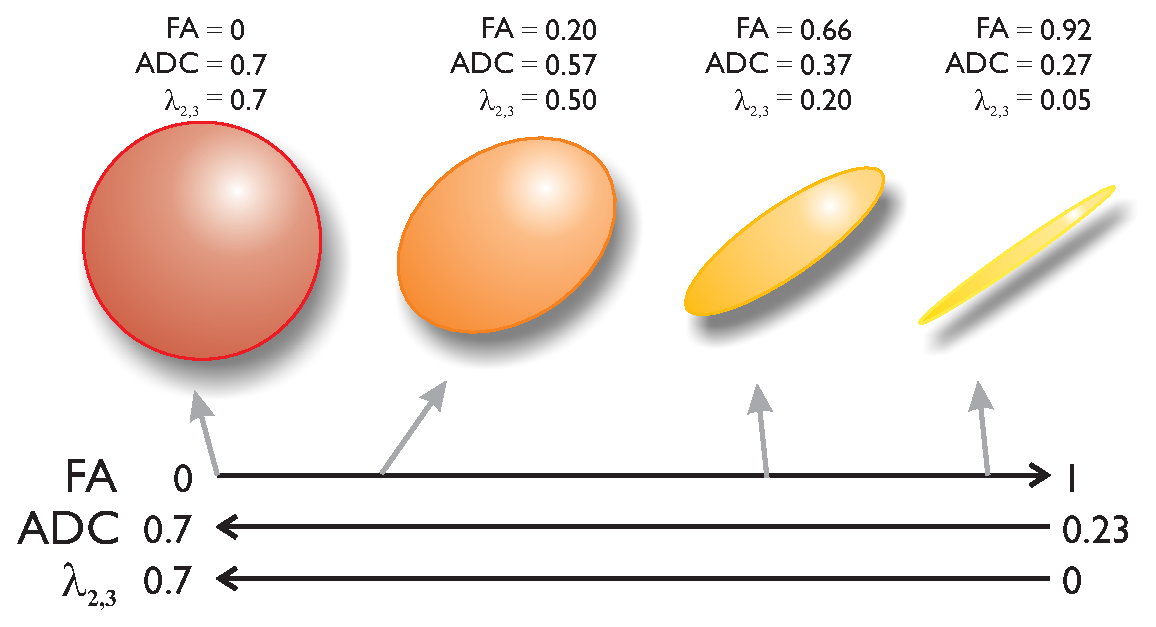
\includegraphics [width=0.7\textwidth]{DTI_ellipsoids_FA.eps}
    \caption{\textbf{Elipsoides tensor de difusión de diferentes grados de anisotropía.} Se muestran cuatro elipsoides del tensor de difusión que van desde isotropía pura hasta anisotropía muy alta. En todos los casos \lone se ha mantenido constante a 0.7. \lperp (es decir, \ltwo, \lthree)  reduce progresivamente, aumentando la anisotropía y reduciendo el ADC. FA es adimensional, ADC y valores propios tienen unidades \Dunits.}
    \label{F:DTI_ellipsoids_FA}
    \end{figg}
\end{figure}

Los índices de anisotropía cuantitativa, así como los valores propios y los componentes tensores individuales, también se pueden mostrar como mapas relacionando la intensidad de la escala de grises con la medida deseada en cada píxel (Figura \ref{F:DTI_quantMaps_anisotropy}). De hecho, cualquier escala de colores se puede utilizar y no se limita a una escala de grises (véase, por ejemplo, la Figura \ref{F:DTI_DWItoTensor})). 

\begin{figure}
\begin{figg}
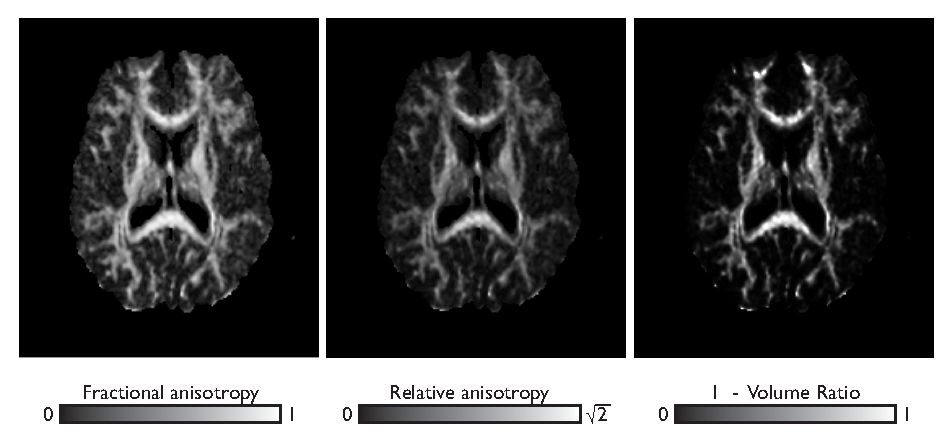
\includegraphics[width=0.7\textwidth] {DTI_quantMaps_anisotropy.eps}
\caption{\textbf{Mapas de anisotropía de difusión cuantitativa.} Se muestran tres medidas de anisotropía de difusión. Observe cómo la sustancia blanca muestra grandes valores en los tres mapas cuantitativos, debido a su alta coherencia arquitectónica.}
\label{F:DTI_quantMaps_anisotropy}
\end{figg}
\end{figure}



Por último, la orientación tridimensional del tensor de difusión también puede visualizarse en imágenes bidimensionales (rebanadas) utilizando diferentes aproximaciones. En el primer enfoque, ejemplificado en la Figura \ref{F:DTI_DWItoTensor}, se visualiza cada elipsoide de difusión (la visualización puede simplificarse mostrando cajas o líneas para representar el tensor). Este enfoque, aunque sea elegante y atractivo a la vista, es extremadamente complicado y difícil de interpretar. Otra reducción de este tema es mostrar $\nu_1$ por píxel como una {\emph quiver-plot}. La principal desventaja de estos métodos es que resulta difícil visualizar la orientación correcta de las flechas/elipsoides cuando están orientadas ortogonalmente al plano que se está viendo (por ejemplo, los elipsóides de difusión de la cápsula interna parecen ser isotrópicos y pequeños en la Figura \ref{F:DTI_DWItoTensor} , panel d). Otros enfoques han producido mapas de escala de grises de los ángulos polares y azimutales de $\nu_1$, que requiere dos mapas para ser vistos simultáneamente \cite{Conturo_1996,Ulug_1994}. Un enfoque inteligente e intuitivo es utilizar el color para representar la orientación de los tractos de materia blanca \cite{Douek_1991,Jones_1997,Coremans_1994,Nakada_1995,Pierpaoli_1997,Jones_1997}. El método más utilizado hoy en día es el propuesto por Pajevic y Pierpaoli \cite{Pajevic_2000}. En este último método, las componentes $x$, $y$ y $z$ de $\nu_1$ se asignan a los componentes rojo, verde y azul de una imagen a color, respectivamente (Figura \ref{F:DTI_colormaps}). Sin embargo, haciendo esto resaltará todos los tensores en la imagen, independientemente de su anisotropía. Dado que las regiones de baja anisotropía pueden tener valores propios ligeramente diferentes sólo debido a las contribuciones de ruido, el valor propio más grande será orientado al azar \cite{Bastin_1998}. Por lo tanto, la corteza y los espacios llenos de LCR parecerán incorrectamente tener una dirección preferida. Con el fin de superar este problema, los componentes del vector se multiplican por algún índice de anisotropía (por ejemplo, FA). Esto coincidirá con la intensidad del píxel con el grado de anisotropía, y el color reflejará la orientación del tensor; además, las regiones de baja anisotropía no abruman la imagen. Otra ventaja de este método es que la codificación de color es independientemente de la orientación de la rebanada.

\begin{figure}
	\begin{figg}
    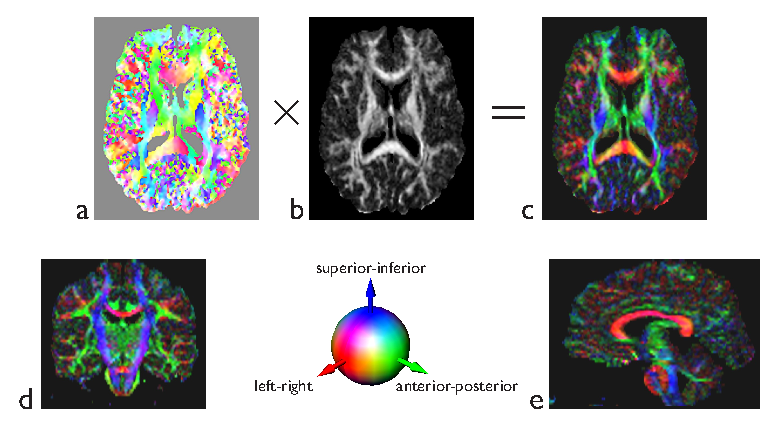
\includegraphics[width=0.7\textwidth]{DTI_colormaps.eps}
    \caption{\textbf{Mapas en color de difusividad principal.} Los componentes $x$, $y$ y $z$ del vector propio principal v 1 se asignan a los componentes rojo, verde y azul de una imagen a todo color (a). Con el fin de resaltar áreas de alta anisotropía, el mapa de color se multiplica por un mapa de anisotropía, en este caso FA (b). El mapa de color resultante (c) muestra la orientación tridimensional del tejido, independientemente de la orientación de la rebanada (c-e).}
    \label{F:DTI_colormaps}
    \end{figg}
\end{figure}




El análisis del tensor de difusión no se limita a las medidas de anisotropía esbozadas anteriormente. Un método intuitivo propuesto por Westin \cite{Westin_1997} representa el tensor como una combinación de sus componentes lineal (CL), planar (CP) y esférico (CE):
\begin{equation}
CL = \frac{\lambda_{1} - \lambda_{2}}{\sqrt{\lambda_1^2 + \lambda_2^2 + \lambda_3^2}}
\end{equation}
\begin{equation}
CP = \frac{2(\lambda_{2} - \lambda_{3})}{\sqrt{\lambda_1^2 + \lambda_2^2 + \lambda_3^2}}
\end{equation}
\begin{equation}
CE = \frac{\lambda_{3}}{\sqrt{\lambda_1^2 + \lambda_2^2 + \lambda_3^2}}
\end{equation}

La normalización por la norma del tensor hace que cada medida oscile entre 0 y 1, y la suma de las tres métricas de forma es la unidad. Cada uno de estos componentes se puede visualizar fácilmente simultáneamente usando un diagrama baricéntrico \cite{Alexander_2000}, y el índice de anisotropía total (CA) se define como la suma de las medidas de forma lineal y plana:

\begin{equation}
CA = CL + CP + 1 - CE
\end{equation}

Este método también puede ser visualizado como mapas cuantitativos (Figura \ref{F:DTI_quantMaps_spher}). La principal desventaja del enfoque de componente de forma es su sensibilidad al ordenamiento de los valores propios, lo cual no es un problema en medidas de anisotropía como FA o RA.

\begin{figure}
	\begin{figg}
    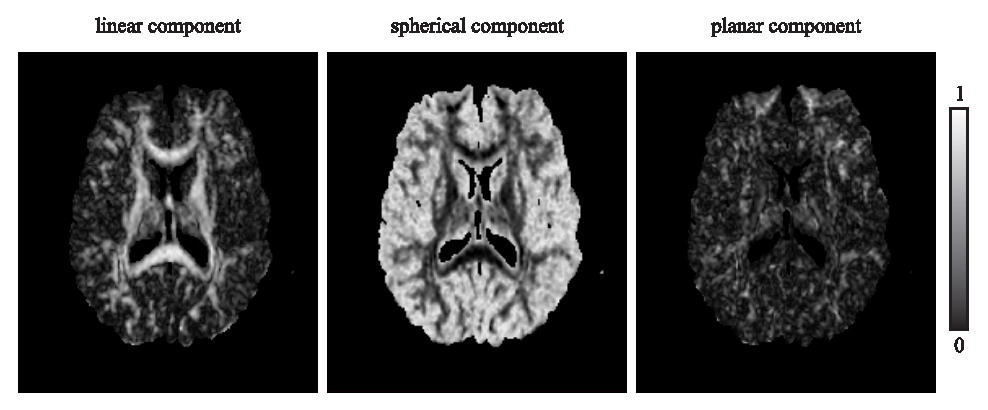
\includegraphics [width=0.7\textwidth] {DTI_quantMaps_spher.eps}
    \caption{\textbf{Componentes geométricos del tensor de difusión.} El tensor de difusión se visualiza como sus componentes esférico, lineal y plano, cuya suma es unidad.}
    \label{F:DTI_quantMaps_spher}
    \end{figg}
\end{figure}


\section{Tractografía}

El tensor de difusión calculado en cada píxel de las imágenes tiene una orientación paralela a la arquitectura de tejidos altamente organizados y coherentes (como la materia blanca y el músculo esquelético). Un conjunto de datos DTI típico incluye varias rebanadas contiguas que forman un volumen, donde el tensor se calcula en cada voxel. La naturaleza tridimensional del tensor y el volumen de las imágenes adquiridas se prestan a la visualización del tejido subyacente utilizando algoritmos informáticos. 

En el caso del cerebro, la sustancia blanca se organiza claramente en fascículos macroscópicos que se distinguen fácilmente en los mapas de color (por ejemplo, el cuerpo calloso es de color rojo brillante cerca de la línea media del panel c en la Figura \ref{F:DTI_colormaps}). El primer enfoque para  aislar haces de fibras individuales utilizó los mapas de color para segmentar voxeles de características similares \cite{Makris_1997}. Poco después, se adaptó una técnica previamente utilizada en la visualización de campos de vectores, llamados líneas de corriente (\textit{streamlines}, en inglés), para la visualización de haces de materia blanca. Varios algoritmos de tractografía  se han desarrollado en la década pasada \cite{Mori_1999,Lazar_2003}, con los primeros informes publicados en 1998 por Basser \cite{Basser_1998} y Jones \cite{Jones_1998}. Esencialmente, en todos los algoritmos se ``siembra una semilla'', en aquellos voxeles con anisotropía por encima de un cierto umbral. Las streamlines se propagan a lo largo de $\nu_1$  por una longitud definida por el usuario, alcanzando el voxel siguiente, donde $\nu_1$ respectivo dicta el siguiente paso a seguir. La propagación de cada streamline continúa  hasta que cumplen un criterio de terminación, que a menudo implica haber alcanzado un voxel con anisotropía baja (para evitar continuar en espacios LCR, corteza o incluso aire), o si la línea se desvía por un ángulo que se considera biológicamente inverosímil.



En el algoritmo de asignación de fibra por seguimiento continuo (``FACT'') \cite{Mori_1999} (Figura \ref{F:DTI_FACT}), todos los voxeles en el conjunto de datos que muestran un valor de FA por encima de un cierto umbral (típicamente en el intervalo de 0.25 a 0.30) son ``sembrados'' y cada línea se propaga según $\nu_1$. Cada vez que la línea se encuentra con el límite entre dos voxeles, pregunta la dirección de $\nu_1$ y FA del voxel al que está apuntando. Si el valor de FA está por debajo de un umbral, o si el ángulo en el que se gira es grande y biológicamente poco probable (por ejemplo,$>70$\textdegree{}) la streamline se trunca. El algoritmo se ejecuta una segunda vez, ya que $\nu_1$ es bidireccional. Decidir la dirección del tracto en las intersecciones del voxel a diferencia de cada paso de longitud fija (que requiere la interpolación del tensor) aumenta la eficacia computacional, aunque ésta segunda alternativa se ha vuelto más popular recientemente. La selección de los umbrales de anisotropía y curvatura es dependiente del usuario y suele adaptarse a la meta en cuestión (es decir, los fascículos de interés). Si se fija el umbral de FA demasiado alto, se minimiza la posibilidad de una propagación errónea a expensas de obtener menos tractos y dificultar la disección. Por el contrario, un umbral de FA muy bajo (por ejemplo $<0.10$) forzará al algoritmo a iniciar la propagación en áreas donde la dirección de difusividad principal podría ser biológicamente sin sentido o determinada por contribuciones de ruido (por ejemplo, en LCR). La misma idea se aplica al umbral de FA de terminación \cite{Mori_2002a,Dauguet_2007}. El umbral de curvatura se hace a menudo muy estricto cuando se analizan tractos con curvatura mínima, como el tracto cortico-espinal. Para el análisis de las fibras U cortico-corticales, el umbral debe ser relajado, ya que estas conexiones se doblan bruscamente dentro de la sustancia blanca subcortical.


\begin{figure}
	\begin{figg}
    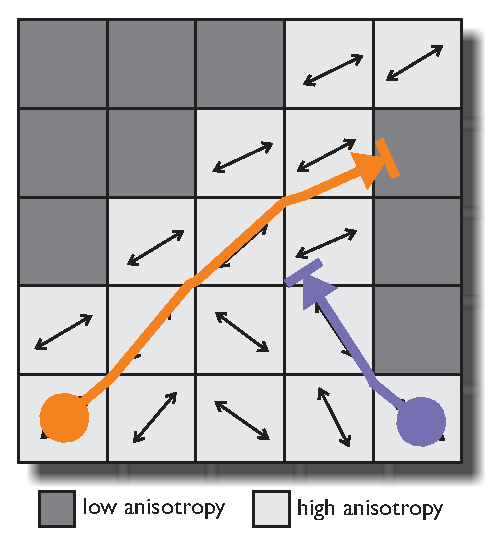
\includegraphics [width=0.7\textwidth] {DTI_FACT.eps}
    \caption{\textbf{Tractografía.} Todos los voxeles con FA alta son ``sembrados''. En este ejemplo bidimensional simplificado, se muestran dos de los tramos resultantes. Las líneas se propagan en la misma dirección que la principal difusividad del voxel (flechas bidireccionales negras), cambiando su rumbo cada vez que encuentran un límite. El tracto naranja se detuvo cuando alcanzó un voxel con anisotropía baja, mientras que el tracto azul se detuvo cuando intentó hacer un giro brusco.}
    \label{F:DTI_FACT}
    \end{figg}
\end{figure}

Todos los algoritmos de propagación de streamlines se pueden iniciar desde regiones de semillas específicas (determinadas por el usuario) o sembrando todo el cerebro. El problema con el primer enfoque es que sólo se puede obtener el mismo número de tractos que el número de semillas, limitando el número de tractos que intersectan el área de interés. Con el segundo enfoque, se obtienen miles de tractos, entonces el usuario selecciona sólo aquellos que pasan por una región específica, proporcionando generalmente mejores resultados, particularmente en áreas de ``ramificación'' de los haces \cite{Conturo_1999}. Con la siembra de todo el volumen, por lo tanto, es absolutamente necesario realizar la disección virtual de los fascículos de interés, sobre la base de un conocimiento {\emph a priori} de su curso. La disección se realiza utilizando operadores booleanos, excluyendo todos los trazos resultantes que no cumplen con los criterios deseados. Dado que la mayoría de los haces de substancia blanca tienen una trayectoria única que no es compartida por los fascículos circundantes, el investigador puede fácilmente proporcionar localizaciones anatómicas a través de los cuales los tractos deben pasar (Figuras \ref{F:DTI_dissection} y \ref{F:DTI_CSTdissection}). La mayoría de los tractos requieren al menos dos regiones de selección de tracto para ser diseccionadas con éxito. Se han publicado pautas para la disección virtual de algunos tractos \cite{Catani_2002,Wakana_2007,catani2008diffusion}, aunque a veces es necesario realizar algunos ajustes adicionales para su representación precisa, debido a diferencias en la calidad de imagen, adquisición, etc.

\begin{figure}
	\begin{figg}
    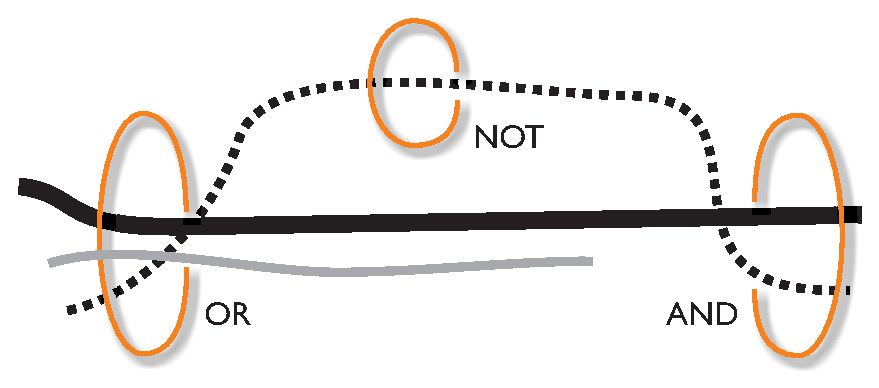
\includegraphics [width=0.7\textwidth]{DTI_dissection.eps}
    \caption{\textbf{Dissección virtual en tractografía.} Después de sembrar todos los voxeles en el volumen con anisotropía alta, sólo se conservan los tractos de interés para su visualización y análisis posterior. Esto se logra colocando estratégicamente áreas a través de las cuales el tramo de interés debe pasar. El operador OR selecciona todos los trazos que pasan por la región. Sin embargo, el delgado tracto gris no pasa a través del operador AND y se desecha. Finalmente, el tramo de puntos, que muestra un camino extraño, se descarta utilizando un operador NOT.}
    \label{F:DTI_dissection}
    \end{figg}    
\end{figure}

Una consideración importante de los algoritmos de propagación de streamlines es que los errores se acumulan a medida que se propagan las líneas. Es decir, para cada voxel hay una contribución de cierto ruido a la estimación del tensor y, a medida que las líneas se propagan y visitan consecutivamente más voxeles, aumenta la probabilidad de que el tracto muestre una desviación aleatoria. La cantidad de incertidumbre en la orientación del tensor se puede calcular y visualizar utilizando el procedimiento {\emph bootstrap} \cite{Jones_2003}. No obstante, se puede utilizar favorablemente la acumulación de errores, ya que los trazos con trayectos incorrectos (determinados por la contribución de ruido) son claramente visibles y pueden eliminarse fácilmente utilizando el operador no booleano.

\begin{figure}
	\begin{figg}
    \includegraphics [width=0.7\textwidth] {DTI_CSTdissection.eps}
    \caption{\textbf{Disección virtual del tracto cortico-espinal.} Todos los voxeles con alta anisotropía son sembrados, resultando en más de 200.000 tractos, 30\% de los cuales se visualizan en el panel a. Con el fin de diseccionar este tracto de interés, los tractos deben pasar por tres regiones (basadas en un conocimiento anatómico \textit{a priori} de la trayectoria del fascículo) identificadas en el panel d. El tracto resultante (b y c), se colorea de acuerdo con la anisotropía (FA). En los paneles b-d, la difusividad principal se denotan con componentes rojos, verdes y azules, superpuestos en imágenes de alta resolución T1 para una mejor apreciación del detalle anatómico.}
    \label{F:DTI_CSTdissection}
    \end{figg}
\end{figure}

Hay otro enfoque de la tractografía que no da lugar a tractos sintéticos que representan la vía de máxima verosimilitud, sino a la probabilidad de que exista una cierta conexión residente en cada voxel, apropiadamente denominada tractografía {\emph probabilística} \cite{Behrens_2003}. Las principales ventajas del método son que caracteriza inherentemente la incertidumbre del modelo tensor, puede utilizarse en áreas de baja anisotropía (como la corteza y la substancia gris subcortical) y es robusta al ruido. La tractografía probabilística se ha utilizado para segmentar con éxito los núcleos del tálamo, basándose en sus proyecciones a la corteza \cite{Behrens_2003a}. La desventaja de este método de tractografía es que encuentra todas las áreas posibles del cerebro con una probabilidad no nula de conectarse a una región de ``semilla'', que a menudo incluye más de un haz de materia blanca. La determinación del umbral inferior de probabilidad de conexión para que un voxel determinado sea considerado como parte de un fascículo es un tema debatible.

\section{Métodos para el análisis cuantitativo del tensor de difusión}

Como se discutió anteriormente, el tensor de difusión y sus medidas derivadas se pueden visualizar como mapas, lo que permite el examen visual de parámetros de difusión cuantitativos. Además, existen métodos para extraer estos parámetros de mapas previamente calculados en uno o varios temas.

\textbf {Regiones de interés.} El análisis de las regiones de interés (ROI, por sus siglas en inglés \index{ROI}) es quizás el más fácil de entender y realizar. En este enfoque, un contorno de dos (o tres) dimensiones se dibuja manualmente alrededor de la estructura de interés. Alternativamente, se puede colocar una forma geométrica de tamaño fijo (por ejemplo, una caja o una esfera) dentro de la estructura de interés. Los voxeles incluidos en la región son consultados para obtener los parámetros deseados y sus valores se promedian con el fin de proporcionar una sola medición por ROI. Dado que todos los mapas de difusión cuantitativos del mismo sujeto están espacialmente alineados, el mismo ROI puede operar en cada uno de los mapas de forma independiente. Es decir, para una estructura particular en un solo sujeto, el operador necesita esbozar la estructura de interés sólo una vez, y obtener los valores de ADC, autovalores, FA, etc. La medición directa de los mapas de difusión cuantitativa proporciona un enfoque para la prueba de hipótesis hechas {\emph a priori}. El inconveniente es que los ROIs se colocan manualmente, lo que hace que este un procedimiento potencialmente tedioso y dependiente del usuario.

\textbf{Análisis basado en tracto.} El tramo de interés se representa utilizando la tractografía en cada sujeto, y todos los voxeles que contribuyen al tracto se tratan como un ROI tridimensional. Este enfoque tiene la ventaja de utilizar la naturaleza semi-automatizada de la tractografía, donde las regiones de selección de trazado pueden definirse de forma poco definida (Figura \ref{F:DTI_CSTdissection}), minimizando la dependencia del método por parte del usuario. Es decir, el usuario no tiene que delinear con precisión una estructura de interés, sino simplemente proporcionar una (o más) áreas amplias a través de las cuales un tramo debe pasar y aprovechar los operadores booleanos (Figura \ref{F:DTI_dissection}) y el conocimiento anatómico de la trayectoria del tracto. Más importante aún,  estructuras curvas o muy delgadas se representan más fácilmente utilizando tractografía que con varios ROIs. Al igual que con los ROI, el investigador debe elegir las estructuras que se analizarán con antelación.

\textbf{Mapeo de parámetros estadísticos.} El análisis de cada estructura sobre cada sujeto puede ser un proceso engorroso y largo si el tamaño de la muestra es grande. Esencialmente, en el mapeo de parámetros estadísticos (SPM, en inglés) los volúmenes cerebrales de los sujetos incluidos en el estudio son transformados espacialmente para que coincidan con una plantilla (o atlas) tan cerca como sea posible, después de lo cual las estadísticas se realizan en cada voxel. Este método fue tomado de la morfometría basada en voxel de los volúmenes cerebrales \cite{Wright_1995,Ashburner_2001} y, aunque es muy atractivo, sufre de varios problemas, el mayor de los cuales es el hecho de que la transformación de la imagen (normalización) de volúmenes individuales a la plantilla nunca es perfecto. En particular, mientras que la forma general, el tamaño y la posición de dos cerebros diferentes pueden ser adecuadamente emparejados, las diferencias individuales sutiles de las estructuras intraparenquimatosas no pueden ser conciliadas \cite{Ashburner_2001}. Con el fin de superar este problema (y para satisfacer los requisitos estadísticos del método), las imágenes normalizadas son generalmente suavizadas utilizando un núcleo gaussiano. Aunque técnicamente es un método analítico independiente del usuario, en realidad el usuario debe seleccionar varios parámetros diferentes, como el nivel de suavizado, que puede influir en gran medida en los resultados y las conclusiones derivadas de ellos \cite{Jones_2005,Jones_2007}. Su mayor ventaja (una desventaja en manos inexpertas) es el hecho de que el investigador no necesita tener una hipótesis {\emph a priori}.

\textbf{Estadísticas espaciales basadas en tractos.} Este es un  enfoque presentado  por Smith {\emph et al}. \cite{Smith_2006}, que minimiza los problemas de SPM y permite que las comparaciones de cerebro completo se realicen sin hipótesis {\emph a priori}. En este método, los mapas FA están alineados con una plantilla, y de la media de todos los mapas FA se obtiene un ``esqueleto'' de los tractos de substancia blanca. Luego, se crea un mapa de esqueleto para cada sujeto proyectando sus mapas de FA en el espacio estándar y rellenando el esqueleto con los valores de FA del centro del tramo más cercano. Esto intenta posicionar todos los sujetos en el mismo espacio, con cada voxel que representa exactamente la misma estructura de la substancia blanca. Después de esto se logra, se pueden realizar estadísticas en cada voxel a través de los sujetos. Al igual que la SPM, se destacan las diferencias significativas, de las cuales la tractografía probabilística puede ser iniciada opcionalmente. La desventaja de este método es que sólo analiza una proporción relativamente pequeña de toda la sustancia blanca disponible, es decir, sólo aquellos voxeles con anisotropía alta. Se pierde información valiosa de un gran número de voxeles en varias estructuras de substancia blanca. Además, muchos tractos de substancia blanca (por ejemplo, el tracto corticoespinal) están organizados somatotópicamente (es decir, tienen un orden anatómicamente definido dentro de ellos), haciendo que el análisis de su porción central sea un sesgo potencial.

\section{Deficiencias de DTI}
\subsection{El modelo}

El modelo de tensor de difusión puede identificar con precisión la arquitectura tisular en los casos en que hay homogeneidad de la estructura dentro del voxel muestreado. Sin embargo, no todas las áreas de la sustancia blanca muestran homogeneidad, particularmente en regiones donde dos o más poblaciones de fibras se cruzan entre sí. En estos casos, el modelo de tensor de difusión no puede identificar la orientación compleja del tejido. La razón detrás de este fracaso es que en DTI, se supone que existe un solo compartimiento de difusión gaussiana dentro de cada voxel. La adición de dos tensores prolatos (es decir, $\lambda_{1} > \lambda_{2,3}$) da como resultado un tensor oblato (es decir,$\lambda_{1} < \lambda_{2} = \lambda_{3}$) (Figura \ref{F:DTI_tensorAddition}). Por lo tanto, el problema reside en el propio modelo, y la sobreestimación del tensor de difusión mediante la adquisición de imágenes con múltiples direcciones de gradiente de difusión no es útil.

Es común encontrar áreas de baja anisotropía dentro de la substancia blanca del cerebro, que erróneamente se podrían considerar como lesiones. Se ha estimado que más del 90\% de los voxeles de substancia blanca del humano presentan más de una población de axones \cite{Jeurissen_2012}.  Por ejemplo, la región donde el fascículo longitudinal superior (orientación antero-posterior) cruza la corona radiata (superior-inferior) y el cuerpo calloso (izquierda-derecha) aparece como un ``agujero'' negro en los mapas FA. Además, dado que la mayoría de los algoritmos de tractografía de propagación de streamlines se detienen cuando alcanzan un área de baja anisotropía, los tractos son truncados típicamente en este punto. La tractografía probabilística, que no está limitada por regiones de baja anisotropía donde la orientación es incierta, avanzará en muchas direcciones, potencialmente amalgamando fascículos dispares.

\begin{figure}
	\begin{figg}
    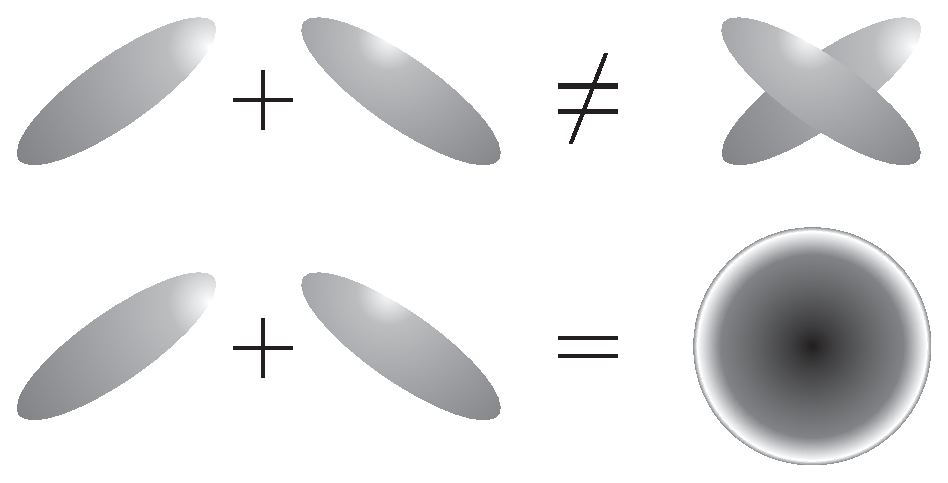
\includegraphics [width=0.7\textwidth] {DTI_tensorAddition.eps}
    \caption{\textbf{Adición de tensores de difusión.} Cuando dos poblaciones de fibras con diferentes orientaciones ocupan el mismo espacio, el modelo tensor no puede diferenciar las dos orientaciones, ya que la adición de dos tensores de difusión prolatos orientados perpendicularmente da lugar a un elipsoide oblato.}
    \label{F:DTI_tensorAddition}
    \end{figg}
\end{figure}

La verdadera función de difusión en las zonas de cruce de fibras es compleja. Por esta razón, se han propuesto  descripciones  del perfil de difusión libres de modelo \cite{Alexander_2002,Tuch_2004}, comúnmente denominadas imágenes de espacio Q o imágenes de difusión de alta resolución angular. En resumen, la función de difusión está relacionada con la señal de RM por la transformada de Fourier con respecto al vector de onda de difusión experimental $q$ (el gradiente de difusión y su dirección) \cite{Stejskal_1965, Tuch_2004}. Los métodos de espacio Q utilizan alta resolución angular a altos valores de $b$ y un gran número de direcciones de gradiente de difusión (generalmente más de 100). La sensibilidad de difusión ($b$) se incrementa para aumentar el contraste entre el componente de difusión rápida de las dos (o más) poblaciones de fibras \cite{Tuch_2003}. El objetivo es muestrear con precisión el perfil de difusión en cada voxel. En el caso de una sola población de fibra, el perfil de difusión se asemeja a un cacahuete (la difusión es mayor sólo en el eje principal del cacahuete), mientras que en el caso de dos o más poblaciones el cacahuete se convierte en una estructura multi-lobulada simétrica similar a una flor. En particular, los picos del perfil de difusión no corresponden a las direcciones de las fibras. Con el fin de obtener estos, se utiliza  la transformación de Funk-Radon \cite{Tuch_2004}. Una vez que se ha encontrado la orientación de las fibras, los algoritmos de tractografía modificada pueden representar fascículos de substancia blanca, incluso en áreas donde se intersectan. Aunque estas mediciones de difusión libres de modelos son muy útiles, no han recibido tanta atención como lo ha hecho DTI, tal vez debido a los tiempos de adquisición muy largos requeridos, la gran cantidad de datos necesarios para recrear el perfil de difusión y, lo más importante, que las medidas escalares derivadas de DTI se interpretan más fácilmente desde un punto de vista biológico. 

Tanto DTI como la Q-ball (o cualquier método de tractografía derivada de DWI) comparten un inconveniente, que es su incapacidad para discernir aferentes de las fibras eferentes. Es decir, mientras que la conectividad entre dos áreas puede inferirse y visualizarse, su direccionalidad sigue siendo desconocida.

\subsection{Artefactos de imagen}
\label{sec:ArtefactosDWI}

Típicamente, los experimentos DTI en humanos usan volúmenes de voxel que varían de 6 a 20 $mm^{3}$. Dada esta restricción, sólo los haces de materia blanca con dimensiones considerablemente mayores que el tamaño del voxel pueden ser identificados y caracterizados correctamente. Por lo tanto, se pueden representar adecuadamente estructuras grandes, como el cuerpo calloso, las cápsulas internas o el fórnix, pero varias conexiones pequeñas pero importantes no pueden identificarse de forma fiable con DTI.

Es importante recordar que la información de los tensores disponibles en cada voxel corresponde al promedio ponderado de todas las clases de tejidos que residen en el mismo. Por lo tanto, si un voxel particular está ocupado por LCR y substancia blanca altamente coherente, el tensor resultante no será altamente anisotrópico, sino algo isotrópico (es incluso probable que tenderá más hacia el caso isotrópico, dada la difusión muy rápida de LCR) \cite{Concha_2005}. De hecho, el {\emph promedio de volumen parcial}, como se conoce como este artefacto, puede reducirse aumentando la resolución de las imágenes (reduciendo efectivamente el tamaño del voxel, minimizando la posibilidad de tener más de un tipo de tejido por voxel). Un aumento en la resolución tiene un alto precio, ya que está inversamente relacionado con la relación señal-ruido con tiempos de adquisición fijos. Existen métodos para eliminar la contribución del LCR en la señal mediante pulsos inversores \cite{Concha_2005}, o su contribución puede estimarse a posteriori \cite{pasternak2009free}.

La resolución de las técnicas actuales de DTI está restringida por la secuencia de generación de imágenes usada para adquirir los datos, que a su vez está restringida por el hardware (particularmente la magnitud de los gradientes). La codificación espacial mediante EPI se utiliza generalmente, ya que permite imágenes muy rápidas, lo cual es absolutamente necesario dado el gran número de imágenes necesarias para construir un volumen de ITD (por ejemplo, con seis direcciones de gradiente de difusión, una imagen ponderada de no difusión por rebanada, ocho promedios y 60 rebanadas: $7×8×60 = 3360$ imágenes) y para minimizar los artefactos de movimiento. El tiempo de adquisición corto alcanzado con EPI se logra utilizando un solo impulso de radiofrecuencia de excitación de spin (es decir, un solo impulso de 90\textdegree{}), después de lo cual se llena la totalidad del \espaciok alternando entre gradientes de codificación de frecuencia positiva y negativa precedido por \textit{blips} del gradiente de codificación de fase (Figura \ref{F:kspace}). El movimiento del paciente se minimiza así, ya que cada imagen es esencialmente una ``instantánea'' de la posición actual.

\begin{figure}
	\begin{figg}
    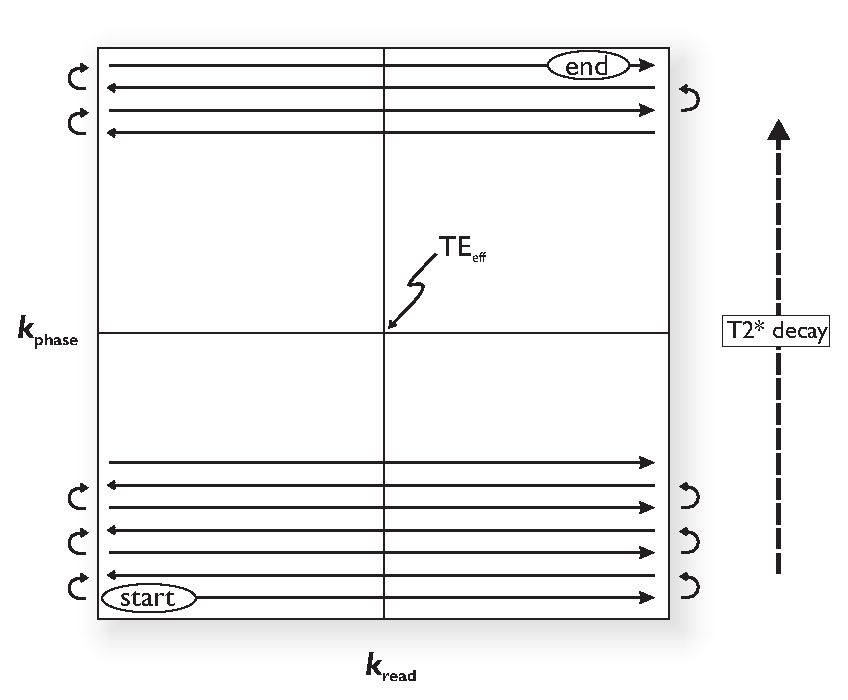
\includegraphics [width=0.7\textwidth]{kspace.eps}
    \caption{\textbf{Trayectoria EPI para la adquisición del \espaciok.} Después de una sola excitación, se adquieren líneas alternas de \espaciok, precedidas por ``blips'' de los gradientes de codificación de fase. El TE efectivo ($TE_{eff}$) está determinado por la línea de adquisición que atraviesa el centro del \espaciok. La señal disponible decae de acuerdo al \Ttwostar del tejido a lo largo de la adquisición del \espaciok.}
    \label{F:kspace}
    \end{figg}
\end{figure}

Por desgracia, la velocidad de adquisición mediante EPI tiene un precio. Dos artefactos muy evidentes vistos en DTI son causados por la secuencia de DWI, ambos de los cuales son aún mayores en fuerzas de campo más altas. El primer artefacto  potencial se llama N/2 o fantasma Nyquist. Las inconsistencias de los ecos pares e impares causan desplazamientos de fase que producen un fantasma desplazado por la mitad de los pixeles de campo de visión (FOV) en la dirección de codificación de fase, en relación con la imagen real. Si el FOV es lo suficientemente grande, estos fantasmas aparecen fuera de la imagen real y no son un problema. Sin embargo, esto no siempre es el caso, para lo cual se han propuesto varios métodos de corrección que adquieren datos de referencia adicionales \cite{Hu_1996} o utilizan esquemas de posprocesamiento \cite{Zhang_2004}. El segundo artefacto se debe a inhomogeneidades de campo magnético que alteran la fase de los giros, con una posterior interpretación errónea de su ubicación en el espacio. La diferencia de susceptibilidad magnética se hace más evidente por el decaimiento \Ttwostar que se produce durante la lectura EPI en la dirección de codificación de fase (Figura \ref{F:kspace}). Las {\emph distorsiones geométricas}, como se conoce a este segundo artefacto, son más aparentes cerca de las interfaces de tejido, sobre todo si poseen susceptibilidades magnéticas muy diferentes, como el aire y el tejido. Por lo tanto, este artefacto es evidente cerca de los senos para-nasales o en la base del cráneo, donde parece que el cerebro ha sido ``aplastado'' (para la codificación de la fase anterior-posterior) o cortado (en la izquierda-derecha de codificación de fase). Al igual que con los artefactos N/2, se han publicado varios métodos que intentan minimizarlo \cite{Weiskopf_2005,Jezzard_1995,Reber_1998}. Dado que el artefacto por inhomogeneidades geométricas se exagera por el decaimiento \Ttwostar durante el llenado del \espaciok, una estrategia simple consiste en  reducir  el número de líneas de \espaciok adquiridas a través de Fourier de fase parcial o imágenes paralelas \cite{Pruessmann_1999}. Otra opción es llenar el \espaciok más lentamente: en un extremo tendríamos la adquisición línea por línea del \espaciok mediante ecos de spin; esto podría acelerarse utilizando turbo-spin echo; un paso atrás del factor máximo de aceleración EPI sería el uso de EPI segmentadas, donde la totalidad del \espaciok se llena en dos o tres TR. Cualquiera de estas estrategias incrementará el tiempo de adquisición con respecto a lo que pueda lograrse mediante EPI. En caso de no poder darse el lujo de adquirir lentamente, uno de los métodos más eficientes y utilizados para la corrección de inhomogeneidades geométricas implica la adquisición de al menos un par de imágenes con llenado del \espaciok de forma inversa (por ejemplo, un volumen con llenado antero-posterior, y un segundo con llenado postero-anterior del \espaciok). Los artefactos mostrarán direcciones inversas entre las dos imágenes, y a partir de ellos puede calcularse un factor de corrección que se aplica al resto de las imágenes \cite{andersson2016integrated}.

Aunque es cierto que el movimiento se minimiza en cada una de las adquisiciones de DWI, el movimiento puede ocurrir entre adquisiciones sucesivas, por lo que es necesario realizar un registro de las imágenes de un set de datos DTI, de manera que la misma región anatómica se represente en las mismas coordenadas a lo largo de todo el set. Este paso puede combinarse con la minimización de artefactos por inhomogeneidades geométricas y corrientes de Foucault (corrientes \textit{eddy}, ver adelante) \cite{andersson2016integrated}.

La segunda fuente de artefactos en DWI son los propios gradientes de difusión. Los gradientes alternantes rápidos producen corrientes adicionales (\textit{eddy}, o de Foucault) que afectan negativamente al campo magnético principal. Los campos magnéticos residuales causados por las corrientes eddy producen distorsiones geométricas. Una forma de minimizarlos es utilizar una secuencia de EPI de un solo disparo, dos veces enfocada, \cite{Reese_2003} (Figura \ref{F:ReeseDTI}). Esta secuencia es una modificación de la secuencia de spin-eco de Stejskal y Tanner (Figura \ref{F:stejskal_sequence}) que separa el par de gradientes de difusión-codificación en dos pares (cada par con su respectivo pulso de reorientación). La descomposición de los gradientes de difusión minimiza las corrientes eddy antes de la lectura EPI, produciendo menos distorsiones geométricas y traducciones de imágenes.

Otro efecto de la codificación espacial mediante EPI es la susceptibilidad a efectos de corrimiento químico (\textit{chemical shift}, ver Capítulo \ref{chapter_espectro}). En particular, la grasa y el agua tienen diferentes frecuencias de resonancia (separadas por 3.3 partes por millón, equivalentes a 210 Hz a 1.5 T), lo que da como resultado un fantasma de imagen derivado de grasa que se desplaza espacialmente (en la dirección de codificación de fase). Este problema se supera fácilmente mediante la utilización de la supresión espectral de grasa antes de la excitación (Capítulo \ref{chapter_secuencias}). En este enfoque, los tejidos grasos se excitan selectivamente utilizando un pulso de radiofrecuencia en resonancia con la grasa, después de lo cual la magnetización transversal residual se estropea (\textit{spoiled}) con un pulso de gradiente (Figura \ref{F:ReeseDTI}). La excitación de las moléculas de agua sigue inmediatamente, con lo que la señal resultante está desprovista de contribuciones de grasa.


\begin{figure}
	\begin{figg}
    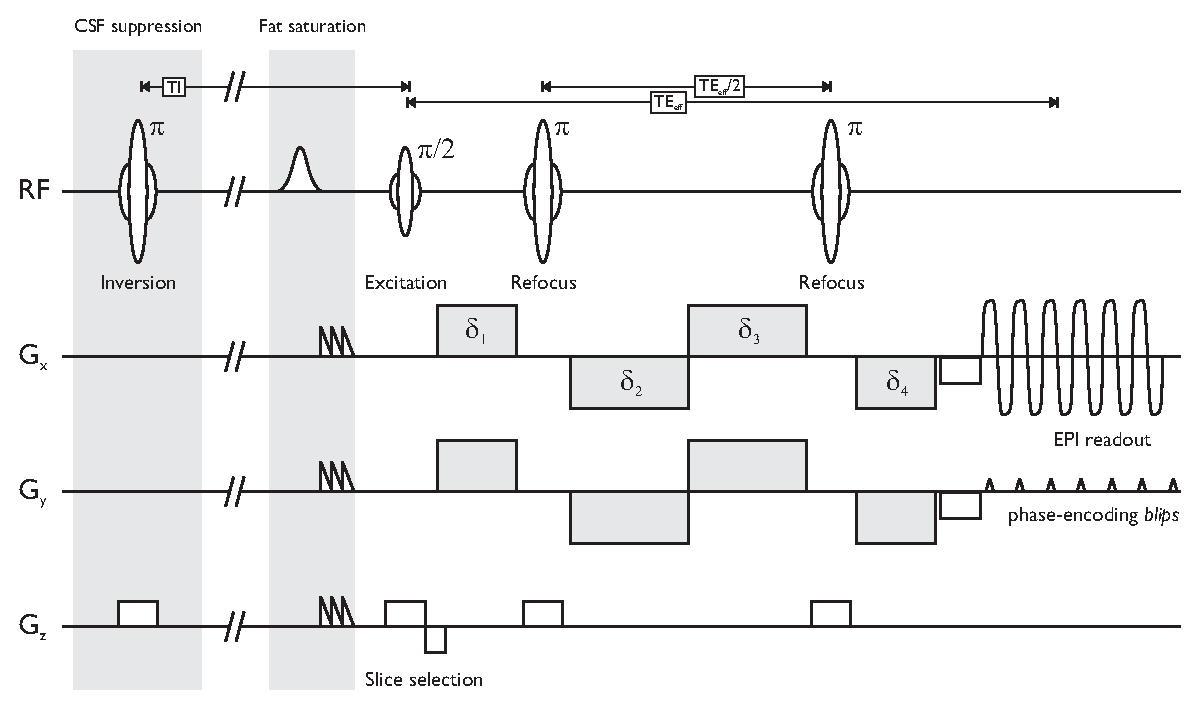
\includegraphics [width=0.7\textwidth] {ReeseDTI.eps}
    \caption{\textbf{Diagrama de secuencia de DTI basado en EPI, doblemente reenfocado, con supresión de LCR.} Un impulso de inversión selectiva se aplica antes del impulso de excitación, separado por un tiempo de inversión (TI) de alrededor de 2200 ms. Esto suprime selectivamente la señal de LCR, basada en su \Tone largo. La supresión espectral de grasa se utiliza antes de la excitación. Se utiliza un conjunto de cuatro gradientes alternantes de sensibilización a la difusión, que compensan sus corrientes eddy, minimizando distorsiones de imagen. Un tren de lectura EPI codifica la información espacial. En este ejemplo particular, los gradientes de difusión se han aplicado en las direcciones $x$ (lectura) e $y$ (fase).}
    \label{F:ReeseDTI}
    \end{figg}
\end{figure}



\section{Cuando el modelo del tensor no es suficiente}

Con el reconocimiento de que el uso de la resolución típica casi el 90\% de los voxels de la sustancia blanca en el cerebro humano contienen fibras cruzadas \cite{Jeurissen_2012} y que el modelo tensor es inadecuado en estas circunstancias (véase la Figura \ref{F:DTI_tensorAddition}), existe una necesidad de encontrar formas alternativas de analizar la señal de difusión que logre capturar  información sobre la microestructura de tejidos complejos. Hay varios métodos para tratar este problema \cite{Jeurissen_2012}, pero todos tienen una cosa en común, y ése es su mayor demanda en términos de adquisición de datos en comparación con DTI. Algunos métodos de espacio q requieren varias decenas de direcciones de gradiente de difusión con uno o más valores $b$ altos ($2.000-50.000 s/mm^{2}$), lo que potencialmente se traduce en tiempos de adquisición prohibitivamente largos ($>$25 min). Afortunadamente, los desarrollos recientes de hardware, diseño de secuencias de pulso y métodos analíticos \cite{Tuch_2002,prckovska_2013} están reduciendo progresivamente el tiempo de escaneo y las alternativas al DTI se están haciendo factibles en el ámbito clínico \cite{Reijmer_2012}. Las ventajas de los enfoques no tensoriales de la tractografía son evidentes e indiscutibles \cite{Farquharson_2012}, y a menudo es absolutamente necesario poder resolver las fibras cruzadas para identificar ciertos fascículos de substancia blanca, como la radiación acústica o los aspectos laterales de la tractografía los tramos córtico-espinales \cite{Behrens_2007}. En el nivel de voxel único es posible obtener métricas de anisotropía de difusión similares a FA, aunque su interpretación biológica no ha sido tan bien estudiada como en el caso del tensor \cite{Concha_Neurosci_2013,rojas2019histological}. 

Exite un gran ímpetu para establecer modelos biofísicos que expliquen la difusión del agua a partir de mediciones derivadas de DWI. Estos modelos buscan, por ejemplo, separar las fracciones de agua  intra-axonal, intra-glial, e intersticial, a la vez que buscan la dirección preferente del agua intra-axonal \cite{panagiotaki2012compartment}.  Mediante combinaciones de parámetros biofísicos pueden estimarse múltiples tensores (u otro tipo de compartimentos) dentro de un mismo voxel. Esto incluso puede llevarse más allá, tratando de encontrar la relación entre la señal asociada al compartimento intra-axonal y la distribución de los diámetros axonales, aunque ésto último ha demostrado ser aún poco preciso \cite{alexander2010orientationally}.

Utilizando un único valor $b>0$  y múltiples direcciones de gradiente, la función de distribución de orientación de fibras (fODF) puede obtenerse a través de la deconvolución esférica \cite{Tournier2004}. La amplitud del fODF es proporcional a la fracción intra-axonal \cite{Raffelt_2012,DellAcqua_2012}. Se han obtenido resultados convincentes por simulación de fibras, y la aplicabilidad de este método se ha demostrado en datos humanos, lo que demuestra que es más sensible que los parámetros DTI para identificar los cambios patológicos en la enfermedad de la motoneurona \cite{Raffelt_2012}. Recientemente, este método fue validado histológicamente en un modelo roedor, donde se observó una clara asociación entre la densidad de axones en el nervio óptico y la amplitud del fODF, viéndose ambas disminuidas en casos de degeneración axonal. Estas métricas son sensibles incluso en voxeles donde existe cruce de fibras, y son capaces de distinguir la población de axones intactos de los degenerados \cite{rojas2019histological}. En ese mismo estudio, se demostró que algunos modelos multi-tensor son capaces también de realizar tal distinción.

La difusión por resonancia magnética es una poderosa herramienta para la evaluación no invasiva de la microestructura de los tejidos; explora ingeniosamente la información relativa al comportamiento de la difusión del agua, empleándola para sondear el entorno microscópico mientras se informa a una escala macroscópica. Proporciona una ventana hacia el reino microscópico en cada voxel de la imagen, mientras que al mismo tiempo permite la identificación  macroscópica de los fascículos de substancia blanca a través de la tractografía. La relativa facilidad con que se puede aplicar para estudiar el cerebro humano la ha hecho muy popular entre los científicos y los médicos, y la técnica está ahora disponible en prácticamente todos los resonadores modernos. Sin embargo, al igual que con cualquier herramienta poderosa, debemos ser conscientes de su alcance y sus limitaciones, teniendo en cuenta que cualquier inferencia sobre la microestructura de los tejidos surge de una medición indirecta y debe considerar todos los factores (biológicos y artificiosos) que pueden influir en la difusión antes de hacer declaraciones categóricas sobre la integridad de la materia blanca.
